\documentclass[a4j]{ujarticle}
\usepackage[dvipdfmx]{graphicx}
\usepackage{url}
\usepackage{bbding}
\usepackage{lscape}
\usepackage[subrefformat=parens]{subcaption}
\usepackage{bm}
\usepackage{amsmath}
% \usepackage{minipage}

\title{進捗報告資料}
\author{安達智哉\\to-adachi@ist.osaka-u.ac.jp}
\date{2019年10月22日}

\begin{document}
\maketitle



\section{Idleタイマの最適化}
以前までの評価において、Idleタイマを適切に設定することにより、CPU負荷およびメモリ使用量の削減が期待できることを示した。
それと同時に、Idleタイマの最適な値は、UEの通信周期やその分布に依存して大きく変化することも示した。

一方で、現実的にはUEの通信周期やその分布は明らかではない。
また、それらは時間とともに変化するものである。
そのため、UEの通信周期やその分布が不明であり、動的に変化するような環境においても、Idleタイマを適切な値に設定するような制御方法が必要となる。そこで本章では、Idleタイマの制御方法に関して述べる。
% 第\ref{sec:IdleTimer_setting}節でIdleタイマの更新タイミングについて述べる。
% 第\ref{sec:hard-state}節でIdleタイマを制御する上での目的関数を定義する。
% 第\ref{sec:control}節で目的関数を最小化するためのIdleタイマの制御方法を述べる。
% \subsection{Idleタイマの更新タイミング}
% \label{sec:IdleTimer_setting}

まず、Idleタイマを各UEに適用するタイミングは、大きく分けて、UEの強制的な状態遷移を引き起こさない方法と引き起こす方法の2種類がある。
まず、UEの強制的な状態遷移を引き起こさない方法として以下の2つが考えられる。
\begin{itemize}
  \item UEがアタッチしたタイミング
  \item UEがデータ送信を行うタイミング
\end{itemize}
次に、UEの強制的な状態遷移を引き起こす方法として以下の2つが考えられる。
\begin{itemize}
\item UEの動作や状態に依存しない、定期的なタイミング
\item 任意のタイミング
\end{itemize}
% さらに、一部の状態のUEに対してのみ強制的に状態遷移を引き起こす方法も考えられる。
% \begin{itemize}
% \item 接続状態およびInactive状態のUEに対しては、MMEが任意のタイミングでIdleタイマを設定できる。一方、アイドル状態のUEは、アタッチもしくはデータ送信のタイミングでIdleタイマを設定する。
% \end{itemize}

それぞれには、メリットデメリットが考えられる。

UEの強制的な状態遷移を引き起こさない方法の場合、更新タイミングがUEの動作に依存するため、新しいIdleタイマをUEに設定するまでにかかる時間がUEごとに異なるという問題がある。
これにより、異なるIdleタイマを持つUEが同時に存在するような状況が発生するため、Idleタイマの制御が複雑になると考えられる。
また、Idleタイマを変更した後、CPU負荷とメモリ使用量に変化が現れるまでに遅延が発生するため、MMEのリソースの制御が難しくなると考えられる。
しかし、アタッチやデータ送信など、UEとMMEが通信するタイミングでIdleタイマの更新を行うため、追加のシグナリングや状態遷移が少なく、オーバヘッドが小さい。

一方、更新タイミングがUEの動作や状態に依存しない場合、Idleタイマを更新するためにUEの状態を変化させる必要がある場合があり、オーバヘッドが大きくなるという問題がある。
具体的には、MMEと通信できない状態にあるUEのIdleタイマを変化させるためには、UEを一度接続状態へと遷移させる必要がある。
この際に、状態遷移に伴うシグナリング処理が発生するため、MMEのCPU負荷が増加する。
しかし、IdleタイマをUEに反映させるまでにかかる時間はUEに依存しないため、全UEのIdleタイマの値を一定期間内で更新できる。
さらに、設定するIdleタイマの値を0にすることで、MMEは任意のタイミングで任意のUEを強制的にアイドル状態へ遷移させることができる。
これにより、UEの強制的な状態遷移を引き起こさない方法の場合と比較してMMEのリソース制御が容易になると考えられる。

% 一部の状態のUEに対してのみ強制的に状態遷移を引き起こす方法の場合のメリットは以下の2点である。
% \begin{itemize}
% \item Idleタイマを更新する際のオーバヘッドを小さく抑えることができる。
% \item Idleタイマを変更した後、CPU負荷とメモリ使用量に変化が現れるまでに遅延を小さくできる。
% \end{itemize}
% この方法では、接続状態およびInactive状態のUEに対してのみ、MMEは任意のタイミングでIdleタイマを設定できる。
% つまり、CPU負荷およびメモリ使用量に影響を与えているUEに対しては、


\subsection{Idleタイマの制御方法(UEの強制的な状態遷移を引き起こさない方法)}
\label{sec:hard-state}
本節では、UEの強制的な状態変化を引き起こさないことを前提にする。
つまり、Idleタイマが切れていないUEを強制的にIdle状態へ遷移させることはないとする。
また、Idleタイマの更新は、UEがデータ送信を行うタイミングで実行するものとする。
MMEはUEを収容するために使用されているCPUおよびメモリリソース量を観測できるものとする。
つまり、UEの収容とは無関係な処理によって発生する負荷を取り除いたCPU負荷およびメモリ使用量を知ることができるとする。
MMEは現在収容されているUE台数を観測できるものとする。

突発的な負荷の増加に対応するという観点から、現在収容しているUEに加え、最も多くのUEを収容できるようなIdleタイマの値が最適と考える。
具体的には、現在収容しているUEと同じ通信周期を持つUEがネットワークに参加すると仮定し、最も多くのUEを追加で収容できるIdleタイマの値を最適と定義する。
また、CPUよびメモリのどちらも過負荷状態でないことは、UEを収容可能であることの必要十分条件であるとする。

まず、UE一台あたりが各リソースに与える負荷の平均を推定する。
現在収容しているUE台数を$N_{\rm UE}$とする。
UE台数が$N_{\rm UE}$、Idleタイマが$T$の時に観測される、CPU負荷およびメモリ使用量をそれぞれ$C_{N_{\rm UE}}(T)$、$M_{N_{\rm UE}}(T)$とする。
この時、UE一台あたりが与えるCPU負荷およびメモリ使用量の平均($C_{1}(T)$、$M_{1}(T)$)は以下の式(\ref{eq:cpu_1})、(\ref{eq:memory_1})で表せる。
\begin{eqnarray}
   C_{1}(T) =& \frac{C_{N_{\rm UE}}(T)}{N_{\rm UE}}\label{eq:cpu_1}\\
   M_{1}(T) =& \frac{M_{N_{\rm UE}}(T)}{N_{\rm UE}}\label{eq:memory_1}
\end{eqnarray}

Idleタイマを$T$とした時に、$N_{\rm UE}$台のUEを収容している状態から追加で収容可能なUE台数を$N_{\rm UE}^{\rm add}(T)$とする。
$N_{\rm UE}^{\rm add}(T)$は、$C_{1}(T)$、$M_{1}(T)$、$C_{N_{\rm UE}}(T)$、$M_{N_{\rm UE}}(T)$、$C^{\rm max}$および$M^{\rm max}$を用いて、以下の式(\ref{eq:UE_add})で表せる。
ここで、$C^{\rm max}$、$M^{\rm max}$はそれぞれシグナリング処理およびUEのセッション情報を保持するために使用可能なCPUリソース量およびメモリリソース量である。
\begin{eqnarray}
   N_{\rm UE}^{\rm add}(T) =& \min \{\lfloor \frac{C^{\rm max} - C_{N_{\rm UE}}(T)}{C_{1}(T)} \rfloor, \lfloor \frac{M^{\rm max} - M_{N_{\rm UE}}(T)}{M_{1}(T)} \rfloor\} \label{eq:UE_add}
\end{eqnarray}
Idleタイマを制御する上での目的関数を以下の式(\ref{eq:objective_function})に示す。
\begin{eqnarray}
  \text{maximize} :& N_{\rm UE}^{\rm add}(T)
  \label{eq:objective_function}
\end{eqnarray}


$N_{\rm UE}^{\rm add}(T)$を最大化するIdleタイマの値が明らかである場合は、その値をIdleタイマに設定すれば良い。
しかし一般的に、UEの台数や通信周期は未知であり時間的に変動するため、$N_{\rm UE}^{\rm add}(T)$を最大化するIdleタイマの値を知ることは難しい。
そのような場合は、$N_{\rm UE}^{\rm add}(T)$を最大化するように、Idleタイマを適応的に制御する必要がある。
具体的には、各リソースの使用量を観測して、$N_{\rm UE}^{\rm add}(T)$を大きくする向きにIdleタイマを変化させる。
このステップを複数回繰り返すことにより、Idleタイマを制御する。
% ここで、Idleタイマを変化させた時に、その効果がMMEのリソースに反映されるまでには一定の時間が必要であることを留意する必要がある。

この時、1ステップごとのIdleタイマの変化量を考える必要がある。
この値を小さく設定すると、最適な値に到達するまでに大きな時間がかかってしまう場合がある。
逆にIdleタイマの変化量を大きく設定すると、Idleタイマが発振する可能性もあり、制御が不安定になる。
また、UEの通信周期によって、Idleタイマが変化した時に各リソースの負荷の変化量が異なる点も考慮する必要がある。
つまり、ネットワークの変化に短い時間スケールで対応しつつ、安定した制御を実現するためには、ネットワークの環境に応じてIdleタイマの変化量を制御する仕組みが必要である。
このような制御には様々な手法が考えられるが、本報告では動作がシンプルであり、汎用性が高いPID制御を用いる。
$T$および$N_{\rm UE}^{\rm add}(T)$をそれぞれ、PID制御における入力値および出力値として捉えることで、Idleタイマの変化量を調整しつつ、最適値に近づけることができる。

まず、PID制御における出力値$y(t)$および目標値$r(t)$を設定する。
以前の評価より、UE台数を固定した時、CPU負荷はIdleタイマの値に対して広義単調減少でありかつ、メモリ使用量はIdleタイマの値に対して広義単調増加であることがわかっている。
このことから、$C_{1}(T)$および$C_{N_{\rm UE}}(T)$は$T$に対して広義単調減少であることがわかる。
同様に$M_{1}(T)$および$M_{N_{\rm UE}}(T)$は$T$に対して広義単調増加であることがわかる。
以上を踏まえて式(\ref{eq:UE_add})を確認すると、$\lfloor \frac{C^{\rm max} - C_{N_{\rm UE}}(T)}{C_{1}(T)} \rfloor$は広義単調増加でありかつ、$\lfloor \frac{M^{\rm max} - M_{N_{\rm UE}}(T)}{M_{1}(T)} \rfloor$は広義単調減少であることがわかる。
ここで、$\lfloor \frac{C^{\rm max} - C_{N_{\rm UE}}(T)}{C_{1}(T)} \rfloor$と$\lfloor \frac{M^{\rm max} - M_{N_{\rm UE}}(T)}{M_{1}(T)} \rfloor$の差分を最小化するような$T$の集合を$\bm{T}$とする。また、$N_{\rm UE}^{\rm add}(T)$を最大化するような$T$の集合を$\bm{T}_{\rm optimal}$とする。すると、$\lfloor \frac{C^{\rm max} - C_{N_{\rm UE}}(T)}{C_{1}(T)} \rfloor$は広義単調増加でありかつ、$\lfloor \frac{M^{\rm max} - M_{N_{\rm UE}}(T)}{M_{1}(T)} \rfloor$は広義単調減少であることを考慮すると、$T\in\bm{T}$であることは$T\in\bm{T}_{\rm optimal}$であるための十分条件になる。

以上の議論のイメージを図\ref{theory_1_all_30s_theory}、図\ref{theory_1_add_C_M}および図\ref{theory_1_add_all}に示す。
図\ref{theory_1_all_30s_theory}はUE台数が500,000台,UEごとの通信周期は10~sから6,000~sの範囲で一様分布とした時の、Idleタイマと各リソース負荷の関係を示したものである。
図\ref{theory_1_add_C_M}は図\ref{theory_1_all_30s_theory}と同じUEを収容した時の、Idleタイマと$\lfloor \frac{C^{\rm max} - C_{N_{\rm UE}}(T)}{C_{1}(T)} \rfloor$と$\lfloor \frac{M^{\rm max} - M_{N_{\rm UE}}(T)}{M_{1}(T)} \rfloor$との関係を示している。
また、図\ref{theory_1_add_all}は図\ref{theory_1_all_30s_theory}と同じUEを収容した時の、Idleタイマと$N_{\rm UE}^{\rm add}(T)$との関係を示している。
図\ref{theory_1_add_all}を見ると、$N_{\rm UE}^{\rm add}(T)$を最大化するIdleタイマの値と$\lfloor \frac{C^{\rm max} - C_{N_{\rm UE}}(T)}{C_{1}(T)} \rfloor$と$\lfloor \frac{M^{\rm max} - M_{N_{\rm UE}}(T)}{M_{1}(T)} \rfloor$の差分を最小化するIdleタイマの値が一致していることが確認できる。


\begin{figure}[htbp]
  \begin{center}
    \begin{tabular}{c}
      \begin{minipage}{1\hsize}
        \begin{center}
          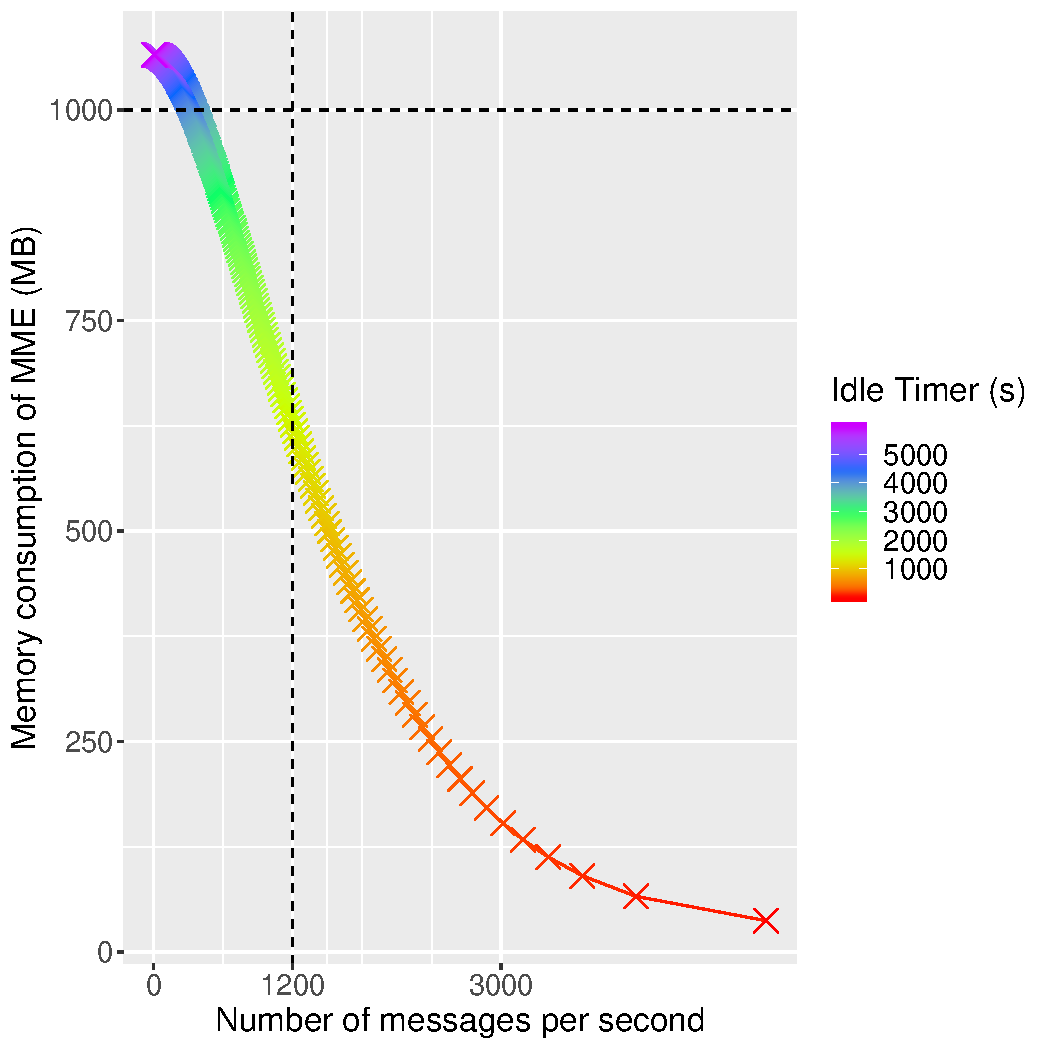
\includegraphics[width=0.6\hsize]{theory_1_all_30s_theory.pdf}
          \caption{Idleタイマに対する,メッセージ処理頻度とメモリ使用量の関係}
          \label{theory_1_all_30s_theory}
        \end{center}
      \end{minipage}
    \end{tabular}
  \end{center}
\end{figure}

\begin{figure}[htbp]
  \begin{center}
    \begin{tabular}{c}
      \begin{minipage}{0.47\hsize}
        \begin{center}
        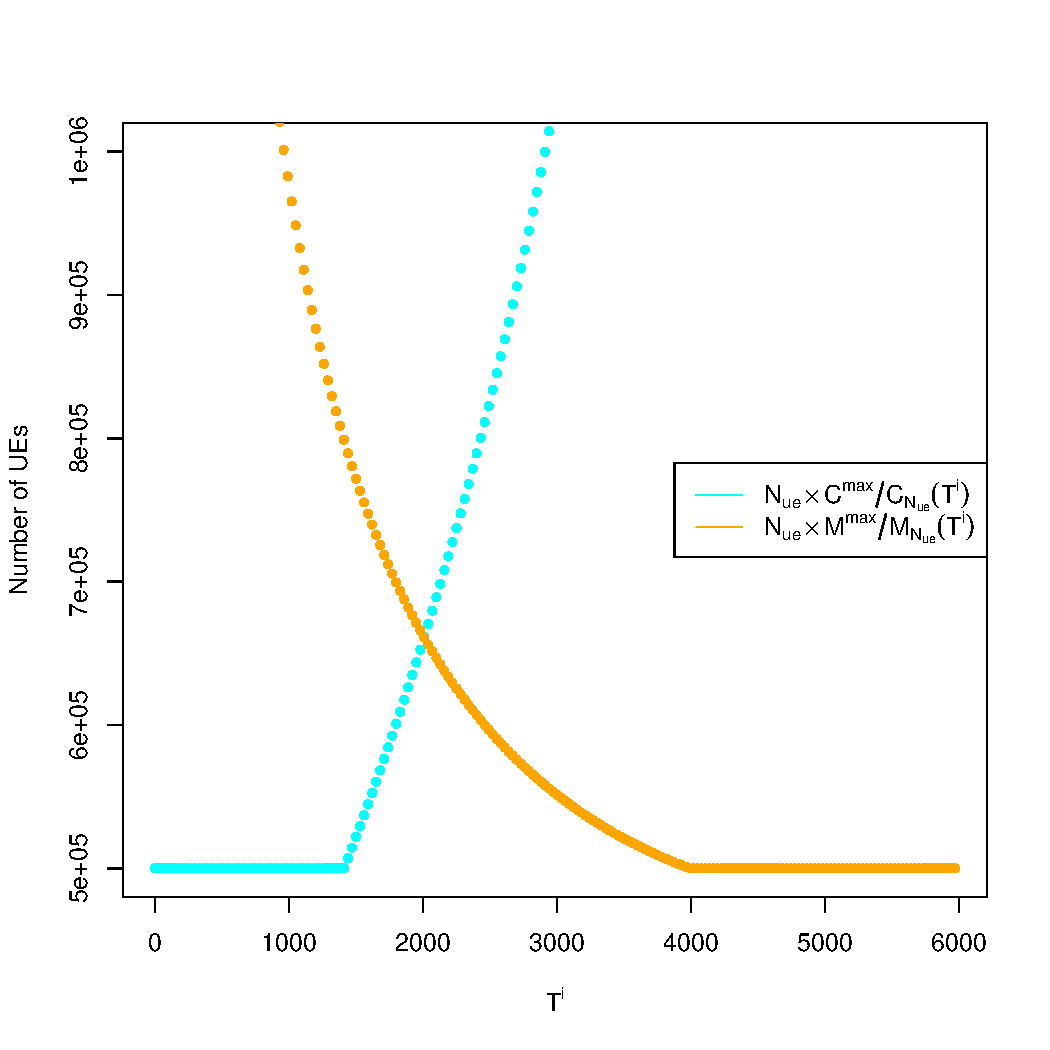
\includegraphics[width=1\hsize]{theory_1_add_C_M.pdf}
        \subcaption{Idleタイマと$\lfloor \frac{C^{\rm max} - C_{N_{\rm UE}}(T)}{C_{1}(T)} \rfloor$と$\lfloor \frac{M^{\rm max} - M_{N_{\rm UE}}(T)}{M_{1}(T)} \rfloor$の関係}
        \label{theory_1_add_C_M}
        \end{center}
      \end{minipage}
      \begin{minipage}{0.47\hsize}
        \begin{center}
        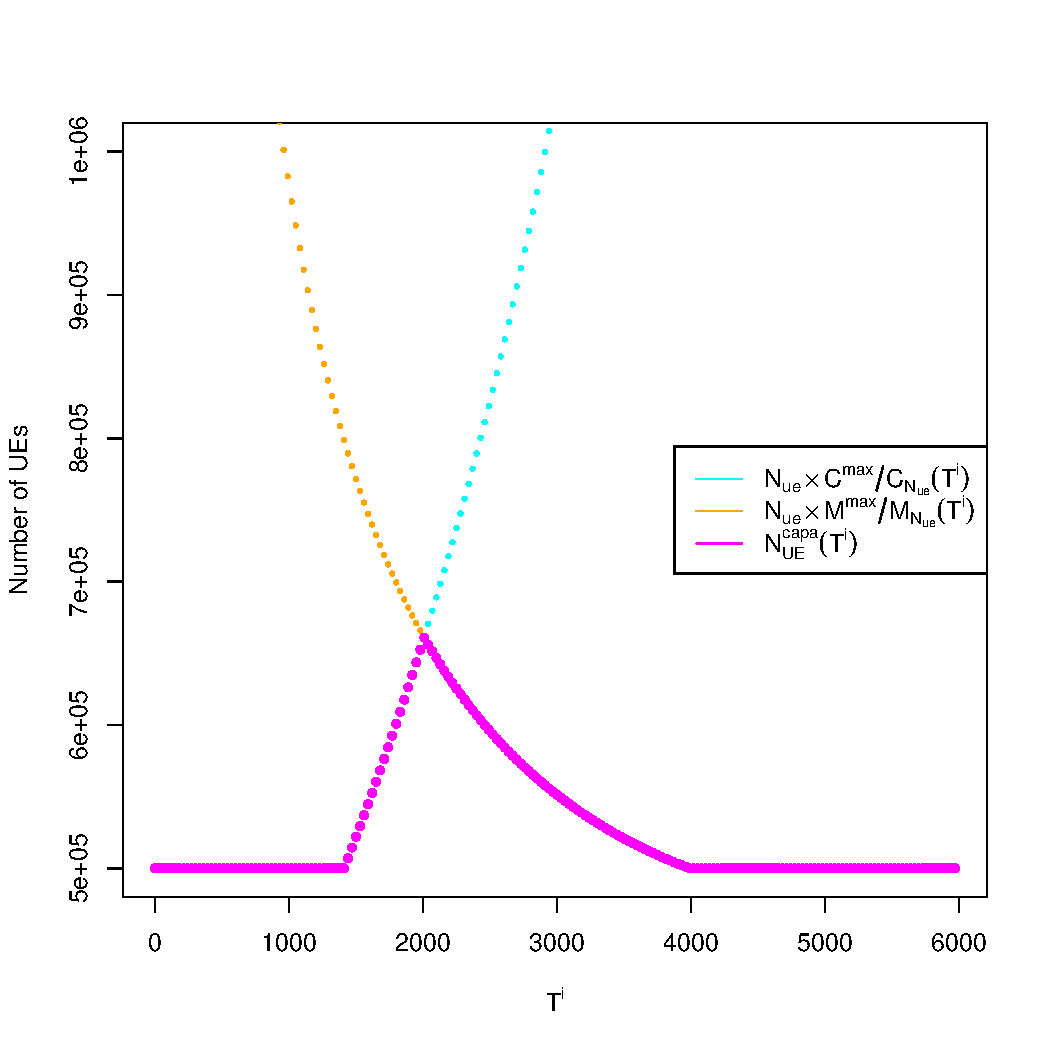
\includegraphics[width=1\hsize]{theory_1_add_all.pdf}
        \subcaption{Idleタイマと$N_{\rm UE}^{\rm add}(T)$の関係}
        \label{theory_1_add_all}
        \end{center}
      \end{minipage}
    \end{tabular}
    \caption{}
  \end{center}
\end{figure}

このことを踏まえ、PID制御における出力値$y(t)$および目標値$r(t)$を以下の式(\ref{eq:PID_y_t})、(\ref{eq:PID_r_t})のように定義する。
$t$は時刻を表す変数である。
\begin{eqnarray}
  y(t) &=& \lfloor \frac{C^{\rm max} - C_{N_{\rm UE}}(T)}{C_{1}(T)} \rfloor - \lfloor \frac{M^{\rm max} - M_{N_{\rm UE}}(T)}{M_{1}(T)} \rfloor
  \label{eq:PID_y_t} \\
  r(t) &=& 0
  \label{eq:PID_r_t}
\end{eqnarray}

時刻$t$における$y(t)$と$r(t)$の差を$e(t)$として以下の式(\ref{eq:PID_e_t})ように定義すると、PID制御における操作量($u(t)$)は以下の式(\ref{eq:PID_u_t})で表せる。
\begin{eqnarray}
  e(t) &=& r(t) - y(t)
  \label{eq:PID_e_t} \\
  u(t) &=& K_p \cdot e(t) + K_i \cdot \int_0^t e(\tau) d\tau + K_d \cdot \frac{de(t)}{dt}
  \label{eq:PID_u_t}
\end{eqnarray}
ここで、$K_p$、$K_i$および$K_d$はそれそれ、比例ゲイン、積分ゲインおよび微分ゲインと呼ばれる定数である。
これらの定数は、$e(t)$およびその積分値、微分値が$u(t)$にどの程度寄与するのかを決定する。

PID制御を機能させるためには、これら3つの定数を適切に設定する必要がある。
しかし、一般的に、これらの定数の最適値を数学的に導出することは困難である。
そのため、試行錯誤を繰り返しながら経験的にパラメータ調整を行う必要があると言われている。
しかし一方で、パラメータの設定方法に関しては、いくつか有名な手順が存在するため、それらに従って設定することもできる。
以下に代表的なパラメータの設定手順を示す。
\begin{itemize}
  \item ジーグラ・ニコルス法
  \item CHR法
\end{itemize}

% (※ $N_{\rm UE}^{\rm add}(T)$を最大化することが本来の目的であるが、最大化問題はそのままではPID制御に落とし込めないと考え、式(\ref{eq:PID_y_t})、(\ref{eq:PID_r_t})に示すように、$N_{\rm UE}^{\rm add}(T)$を用いない形で、出力値および目標値を定義した。本節の第4段落で述べている通り、目的関数は異なるが得られる結果は正しい値であると思われる。)

\subsection{Idleタイマの制御方法(UEの強制的な状態遷移を引き起こす方法)}
\label{sec:soft-state}
現在検討中である。
% 本節では、UEの強制的な状態変化を引き起こすことを前提にする。
% つまり、Idleタイマが切れていないUEを強制的にIdle状態へ遷移させることが可能である。
% また、MMEはCPUおよびメモリリソースの使用量および、現在収容しているUE台数を観測できるものとする。
%
% 第\ref{sec:hard-state}節と同様に、現在収容しているUEに加え、最も多くのUEを収容できるようなIdleタイマの値が最適と考える。
%
% 本節は第\ref{sec:hard-state}節と異なり、UEを強制的にIdle状態へ遷移させることが可能であるため、短期間にメモリ使用量を削減することが可能である。
% そこで、常にメモリに使用量が大きい状態にしておき、UEの増加に応じて一部のUEをIdle状態へ遷移させるような制御が良いと考える。
% 例えば、Idleタイマとシグナリング頻度およびメモリ使用量の関係が図\ref{theory_1_all_30s_theory}のようになる場合、メモリ使用量がメモリ容量を超えない範囲で閾値を設定する。
% そして閾値を超えないギリギリの値(約4,000~s)をIdleタイマに設定する。
% そして、UE台数が増加し、メモリ使用量が増加した場合には、Idleタイマを小さくする。
% 具体的には、メモリ負荷が閾値を下回るまで、最後のデータ送信時刻が古いUEから順にIdle状態へ落としていく。
% そして、メモリ負荷が解消された時に、Connected Inactive状態を維持しているUEのなかで、最後のデータ送信の時刻が最も古いUEを参考にし、新しいIdleタイマを設定する。

\subsection{シミュレーション環境}
\label{sec:simulation_system}
Idleタイマの制御方式の妥当性を評価するためには、UEおよびMMEの動作をシミュレートする必要がある。
UEのシミュレートとは、各UE1台ごとの状態や状態遷移、データ送信等の挙動を再現することである。
MMEのシミュレートとは、全UEの状態および状態遷移から、MMEに発生する負荷を再現することである。
Idleタイマの制御機能とは、上述のシミュレータからMMEの負荷とUE台数を取得し、Idleタイマを制御し、更新されたIdleタイマを上述のシミュレータへ出力する機能である。
Idleタイマの制御機能およびMMEとUEのシミュレータを図\ref{Simulation_UML}のクラス図に示す。

UEのシミュレートはUEシミュレータというクラスで実装する。
UEシミュレータは、各UEの状態や状態遷移、データ送信等の動作をシミュレートする。
これは、UE台数分のインスタンスを生成し、各インスタンスが特定のUEの通信周期やIdleタイマを保持することにより実現する。

MMEのシミュレートはMMEシミュレータというクラスで実装する。
MMEシミュレータは全UEのリストを保持しており、そのリストを参照することにより、各UEの状態および状態遷移を取得する。
そしてそれらの情報から、CPU負荷とメモリ使用量をシミュレートする。

最後にIdleタイマの制御機能は、Idle Timerコントローラというクラスで実装する。
Idle Timerコントローラは、``Idleタイマの更新()"というメソッドを持つが、このメソッドの実装は事前に決定したIdleタイマの制御アルゴリズム(PID制御など)に依存する。
このクラスでは、MMEシミュレータからMMEの負荷とUE台数を取得し、Idleタイマの制御に用いる。
% それ以外の情報(UEの通信周期など)にはこのクラスからはアクセスできない。

\begin{figure}[htbp]
  \centering
  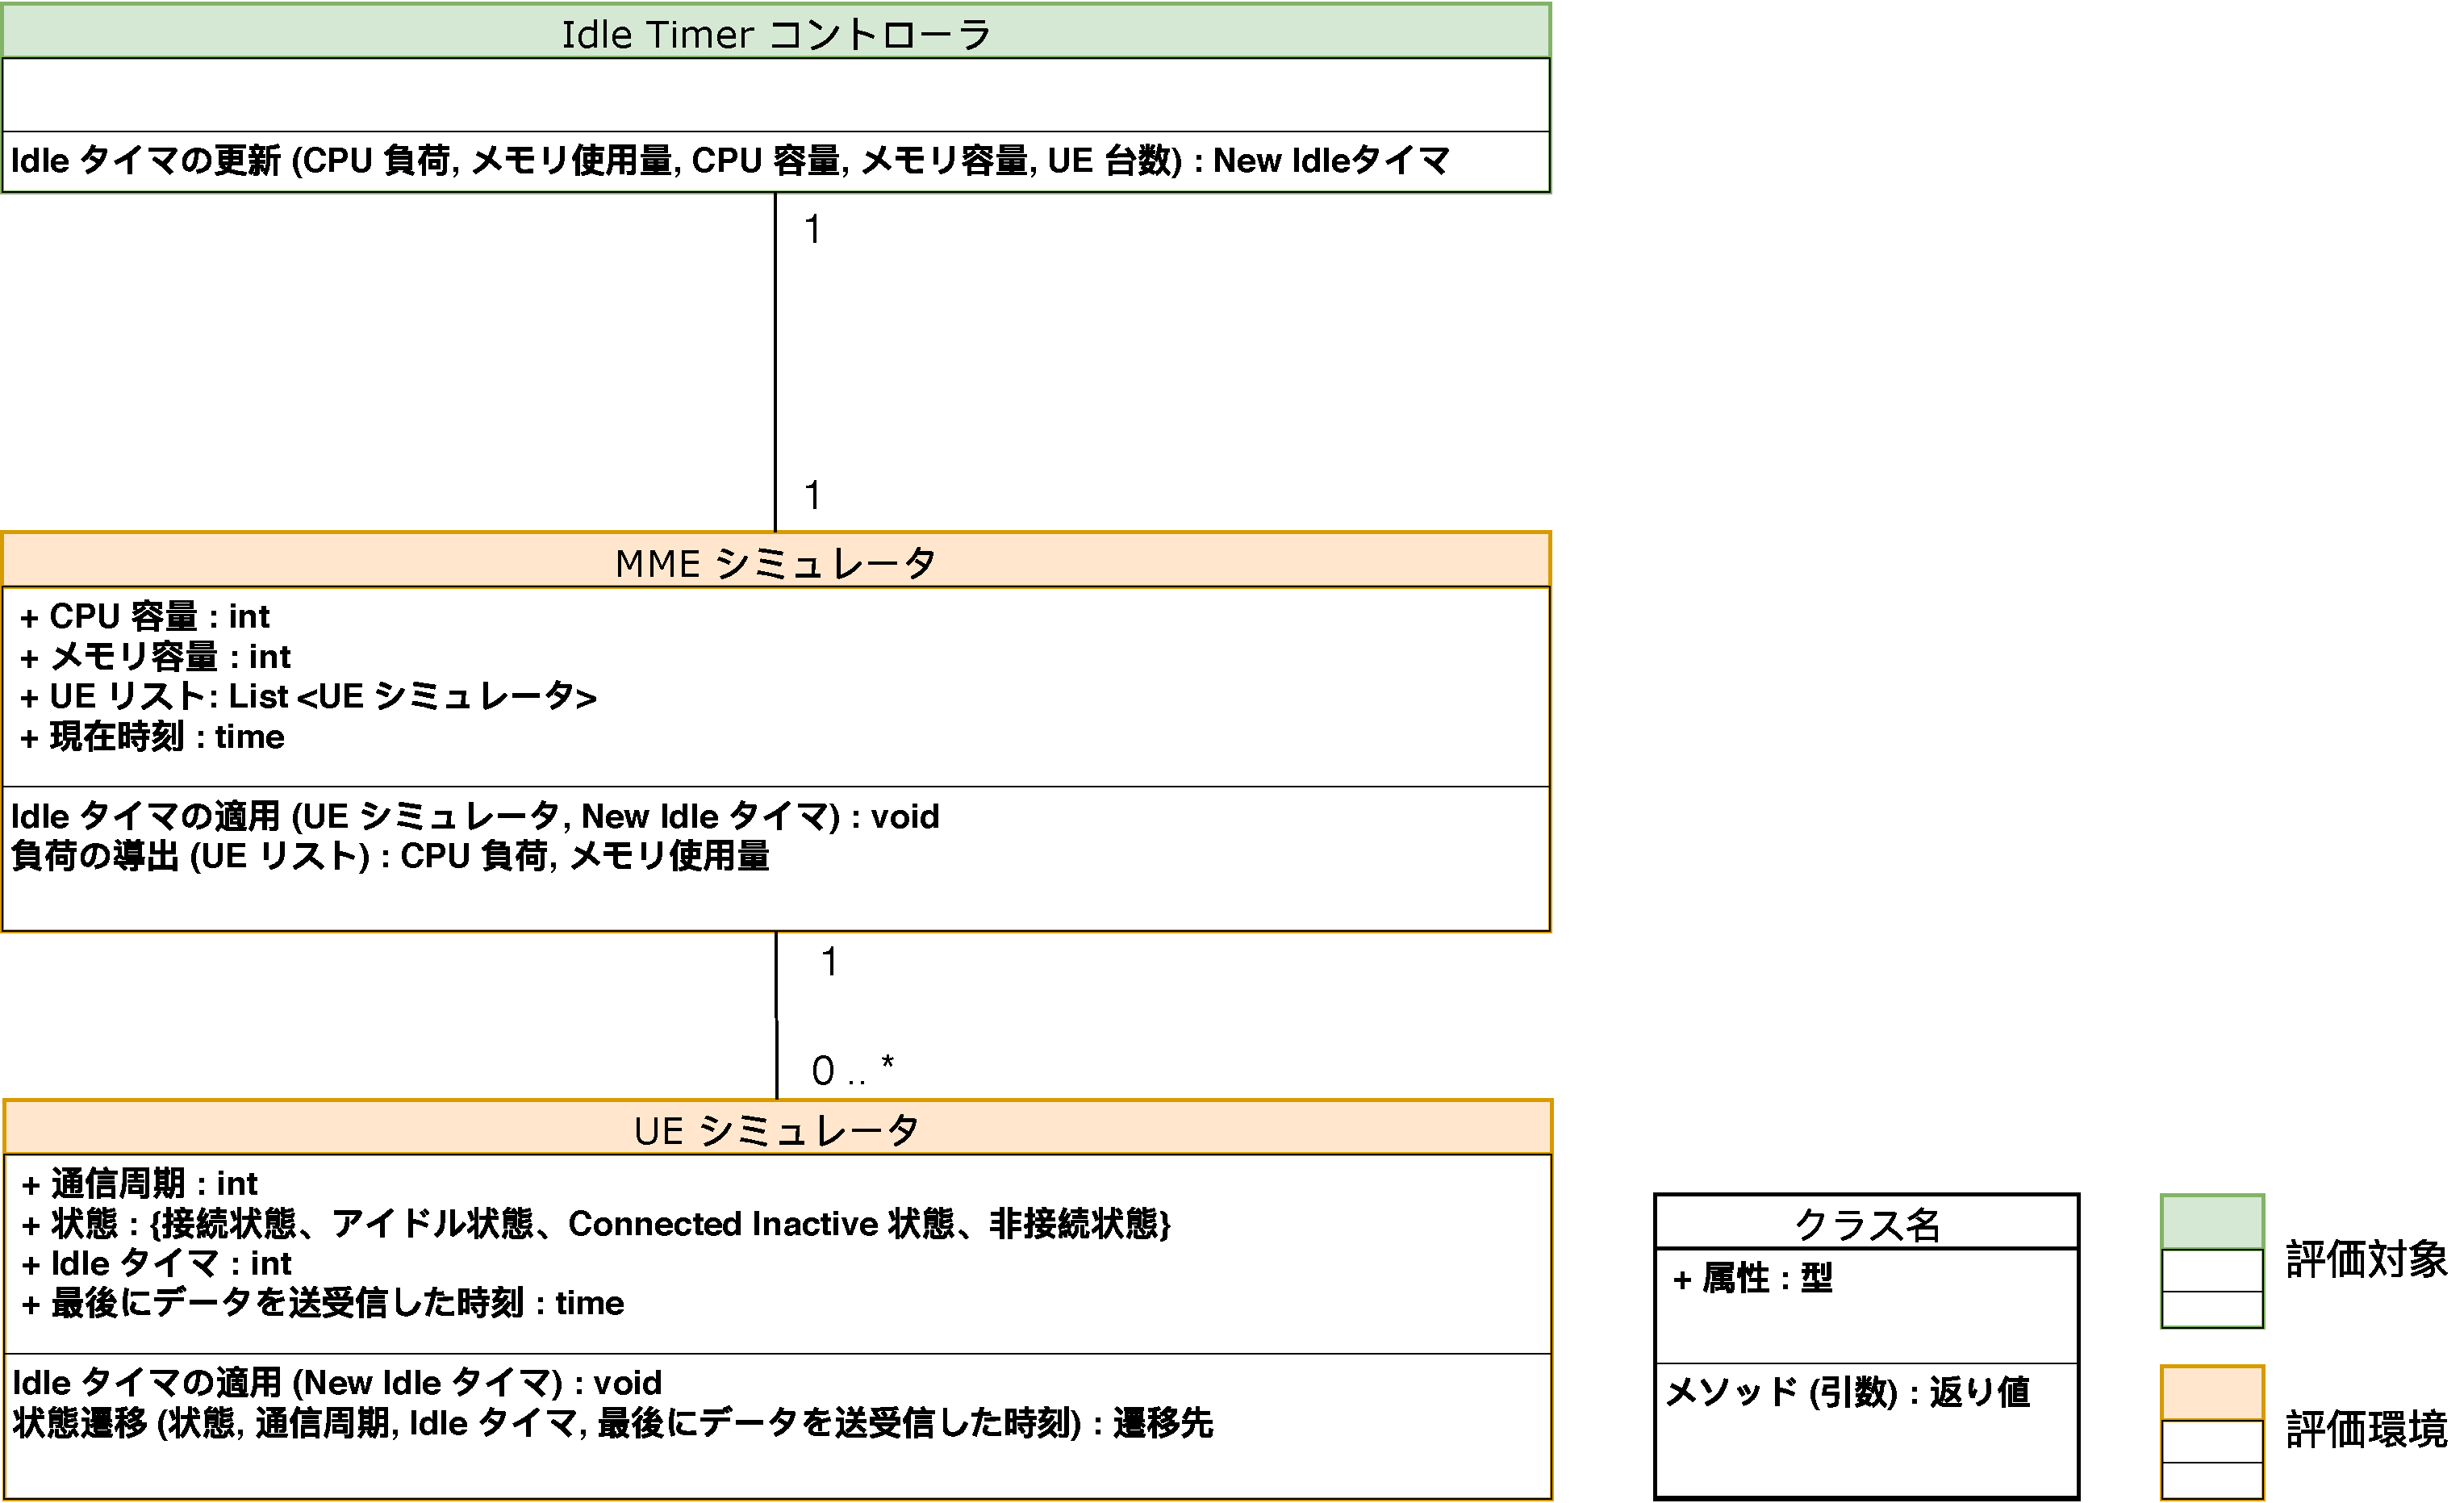
\includegraphics[width=1.0\hsize]{Simulation_UML.pdf}
  \caption{Idleタイマに対する,メッセージ処理頻度とメモリ使用量の関係}
  \label{Simulation_UML}
\end{figure}
\clearpage


\subsection{シミュレーション環境の動作環境}
\label{sec:simulation_program}
第\ref{sec:simulation_system}節で述べたシミュレーション環境を実装した。
評価を行う前に、MMEの負荷を正しくシミュレートできているかを以下の3つのシナリオで確認した。

\subsubsection{シナリオ~1}
シナリオ1では、UE台数を1台とし、その通信周期は20 sとした。
また、タイムステップ1で最初のデータ送信が発生するものとする。
その他のパラメータは表\ref{table:parameter}の通りとし、1タイムステップの長さは1~sとした。
今後の研究ではIdleタイマの制御を行う予定だが、今回はシミュレータの動作確認が目的であるため、Idleタイマは15~sで固定している。
\begin{table}[]
  \centering
  \caption{パラメータ設定}
  \label{table:parameter}
  \begin{tabular}{c|l}
    \hline
    Parameter  & Numerical setting \\\hline \hline
    $T^{\rm ci}$ & 10~s\\
    $s_{\rm MME}^{\rm c \to \rm c}$ & 0~messages\\
    $s_{\rm MME}^{\rm ci \to \rm ci}$ & 0~messages\\
    $s_{\rm MME}^{\rm c \to \rm ci}$ & 0~messages\\
    $s_{\rm MME}^{\rm ci \to \rm c}$ & 0~messages\\
    $s_{\rm MME}^{\rm ci \to \rm i}$ & 5~messages\\
    $s_{\rm MME}^{\rm i \to \rm c}$ & 5~messages\\
    $m^{\rm c}_{\rm MME}$ & 17878~bits\\
    $m^{\rm ci}_{\rm MME}$ & 17878~bits\\
    $m^{\rm i}_{\rm MME}$ & 408~bits\\
    $C^{\rm max}$ & 1200~messages/s\\
    $M^{\rm max}$ & 1,000~MB\\
    $d_h$ & 1 \\\hline
  \end{tabular}
\end{table}

図\ref{scenario_1_signaling_and_memoryload_vs_timeStep}に、タイムステップ毎のMME負荷を示す。
横軸がタイムステップ、縦軸がメッセージ処理数およびメモリ使用量である。
また、図\ref{scenario_1_stateBreakdown}では、各状態に存在するUE台数タイムステップ毎に示している。
図\ref{scenario_1_signaling_and_memoryload_vs_timeStep}と図\ref{scenario_1_stateBreakdown}を見ると、UEがアイドル状態から接続状態へ遷移するタイミングおよびConnected Inactive状態からアイドル状態へ遷移するタイミングでメッセージ処理が発生していることがわかる。
また、UEが接続状態およびConnected Inactive状態である時にメモリ使用量が増加し、アイドル状態である時にメモリ負荷が減少していることがわかる。

\begin{figure}[htbp]
  \begin{center}
    \begin{tabular}{c}
      \begin{minipage}{0.47\hsize}
        \begin{center}
        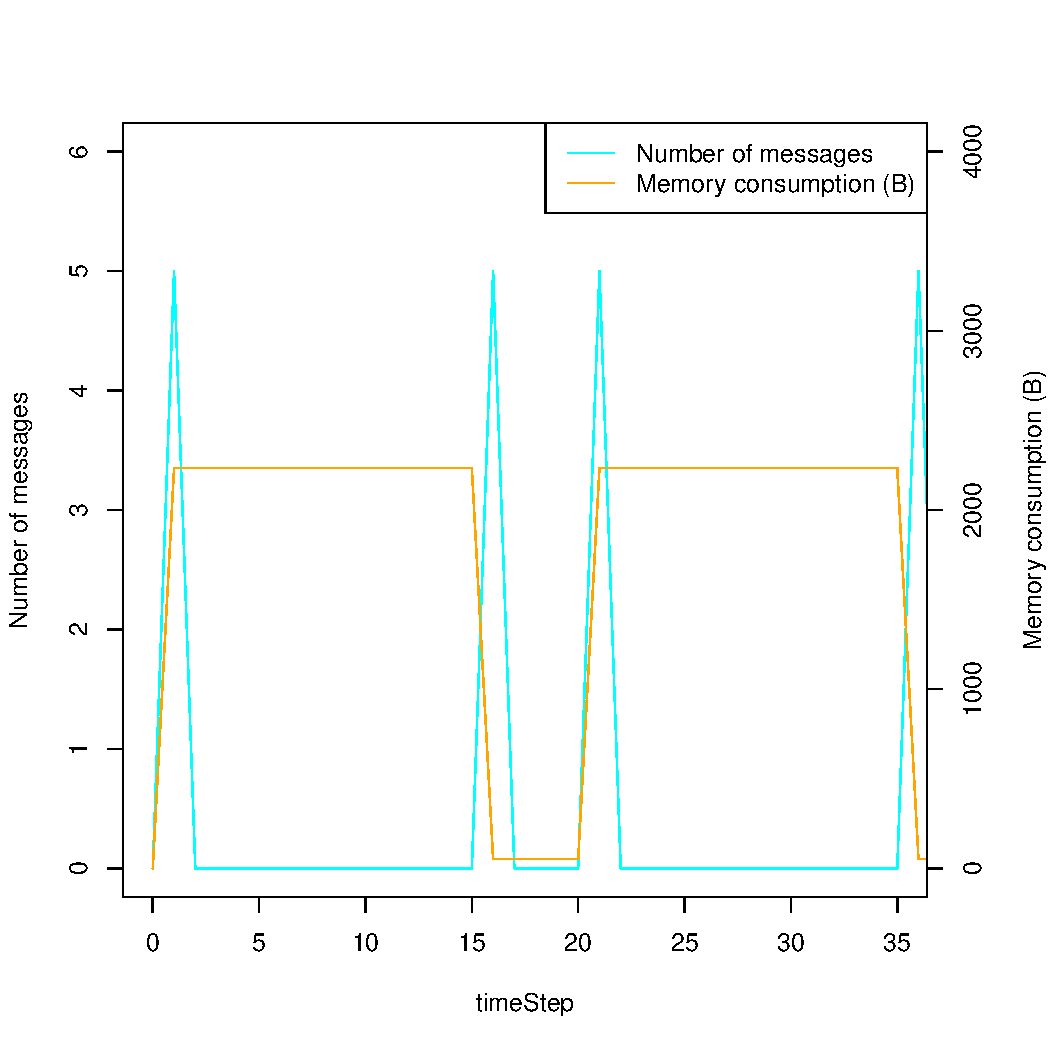
\includegraphics[width=1\hsize]{scenario_1_signaling_and_memoryload_vs_timeStep.pdf}
        \subcaption{メッセージ処理数とメモリ使用量の変化(シナリオ~1)}
        \label{scenario_1_signaling_and_memoryload_vs_timeStep}
        \end{center}
      \end{minipage}
      \begin{minipage}{0.47\hsize}
        \begin{center}
        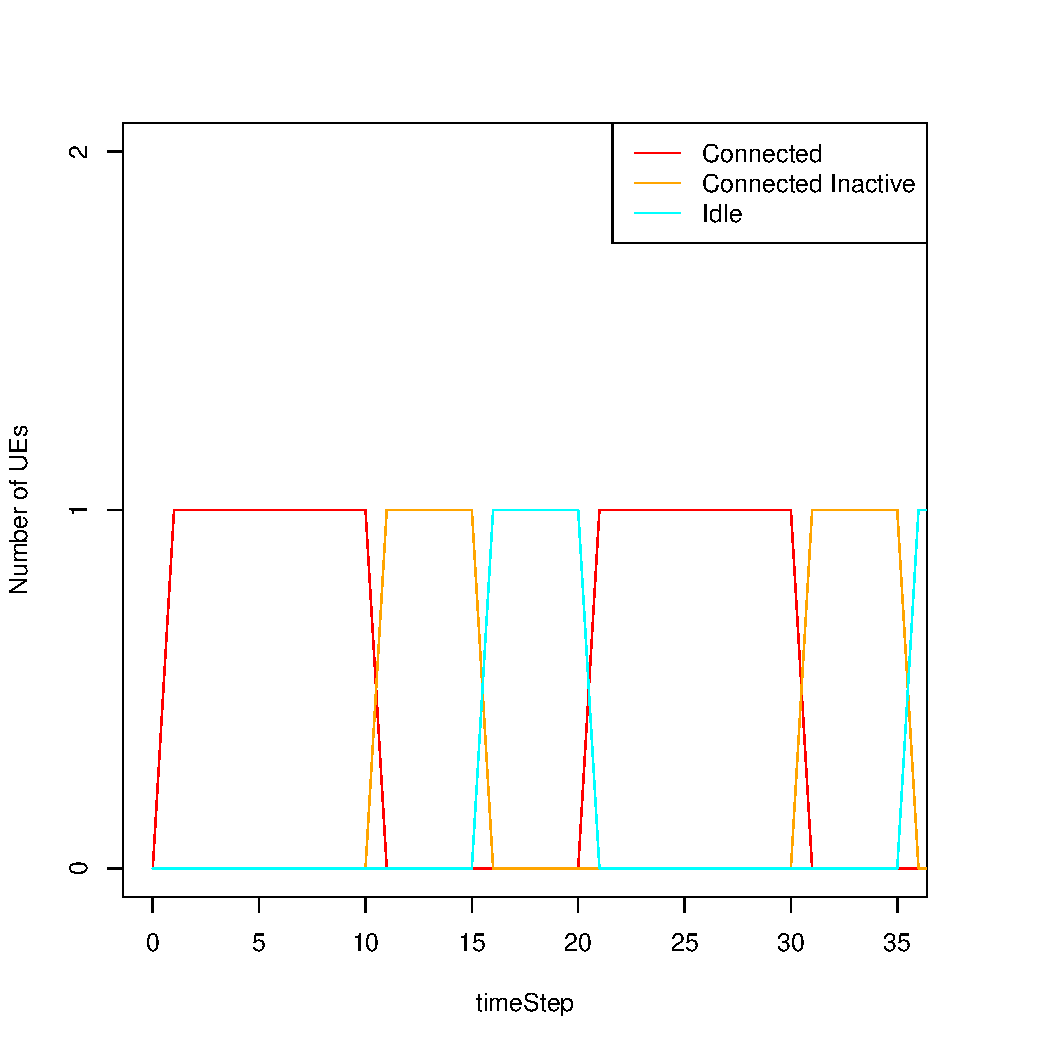
\includegraphics[width=1\hsize]{scenario_1_stateBreakdown.pdf}
        \subcaption{各状態に存在するUE台数の変化(シナリオ~1)}
        \label{scenario_1_stateBreakdown}
        \end{center}
      \end{minipage}
    \end{tabular}
    \caption{}
  \end{center}
\end{figure}


\subsubsection{シナリオ~2}
シナリオ2では、UE台数を約1,036,800台とし、それらの通信周期は1~dayとした。%1036800
また、UEの通信タイミングは理想的に分散している。
その他のパラメータは表\ref{table:parameter}の通りとし、1タイムステップの長さは1~sとした。
Idleタイマは600~sで固定している。

図\ref{scenario_2_signaling_and_memoryload_vs_timeStep}に、タイムステップ毎のMME負荷を示す。
横軸がタイムステップ、縦軸がメッセージ処理数およびメモリ使用量である。
また、図\ref{scenario_2_stateBreakdown}では、各状態に存在するUE台数タイムステップ毎に示している。
シナリオ~1と比較するとMMEの負荷が一定であることがわかる。
なぜなら、UEの通信タイミングが理想的に分散しているため、タイムステップに依存せず、常に一定の台数のUEがデータ送信を行う状態遷移を行うためである。
また、MMEの負荷やUEの状態は正しい値であることを確認した。
\begin{figure}[htbp]
  \begin{center}
    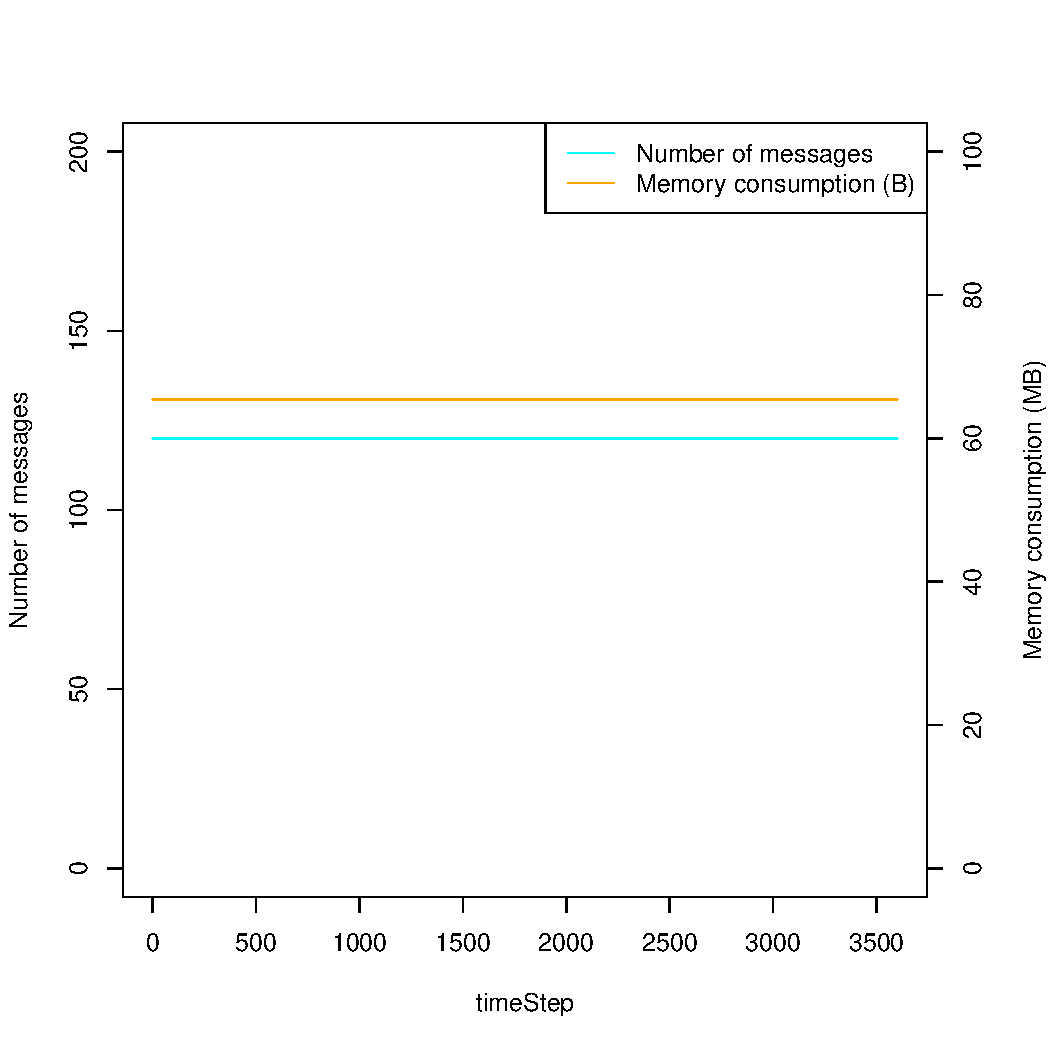
\includegraphics[width=0.6\hsize]{scenario_3_signaling_and_memoryload_vs_timeStep.pdf}
    \caption{メッセージ処理数とメモリ使用量の変化(シナリオ~2)}
    \label{scenario_2_signaling_and_memoryload_vs_timeStep}
  \end{center}
\end{figure}
\begin{figure}[htbp]
  \begin{center}
    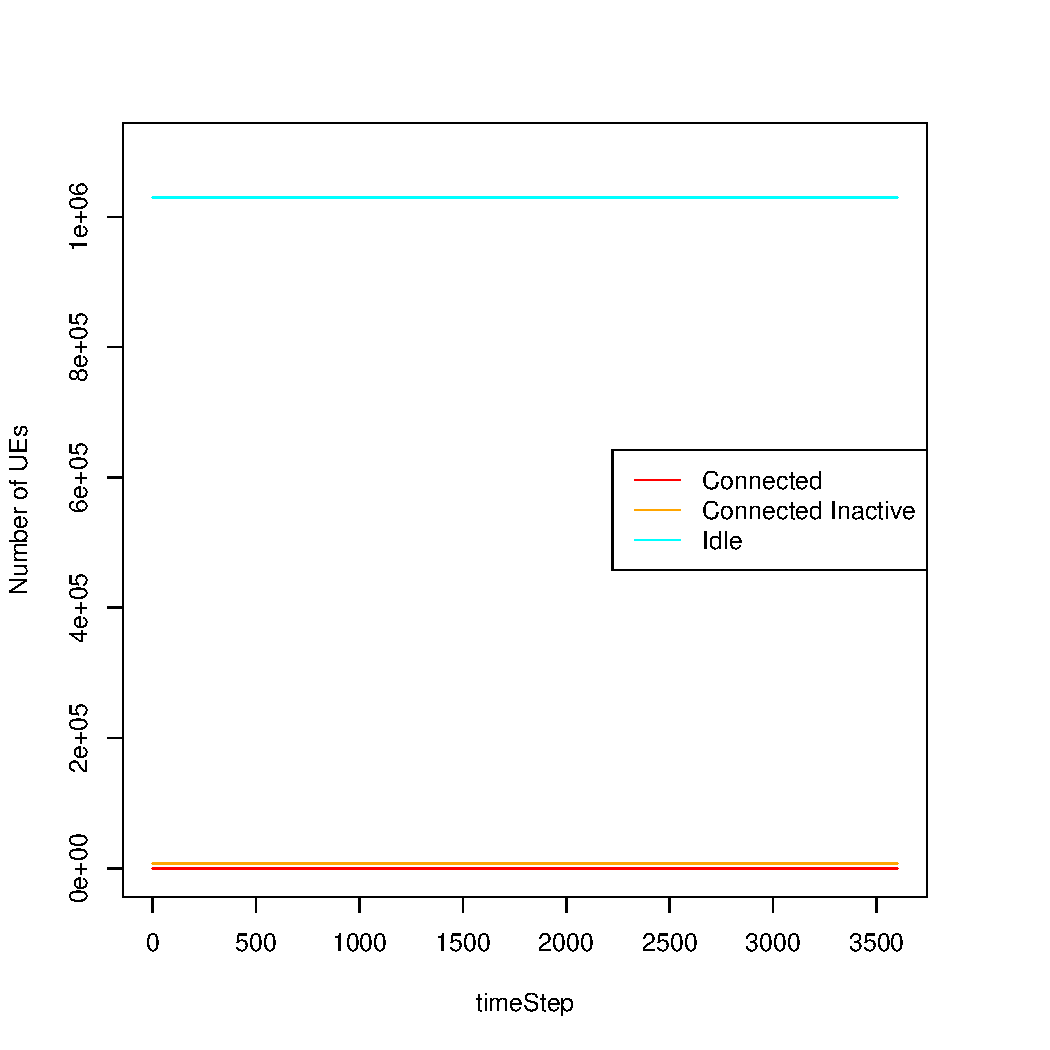
\includegraphics[width=0.6\hsize]{scenario_3_stateBreakdown.pdf}
    \caption{各状態に存在するUE台数の変化(シナリオ~2)}
    \label{scenario_2_stateBreakdown}
  \end{center}
\end{figure}


\subsubsection{シナリオ~3}
シナリオ3は、途中でUEが増加するシナリオである。
初期状態のUE台数は86,400台である。
タイムステップ21,600から43,200の間に86,400台のUEが新しく追加され、UE台数は172,800台に増加する。
全てのUEの通信周期は1~dayとした。%1036800
また、初期状態では、UEの通信タイミングは理想的に分散している。
その他のパラメータは表\ref{table:parameter}の通りとし、1タイムステップの長さは1~sとした。
Idleタイマは3600~sで固定している。

図\ref{scenario_3_signaling_and_memoryload_vs_timeStep}に、タイムステップ毎のMME負荷を示す。
横軸がタイムステップ、縦軸がメッセージ処理数およびメモリ使用量である。
また、図\ref{scenario_3_stateBreakdown}では、各状態に存在するUE台数タイムステップ毎に示している。

\begin{figure}[htbp]
  \begin{center}
    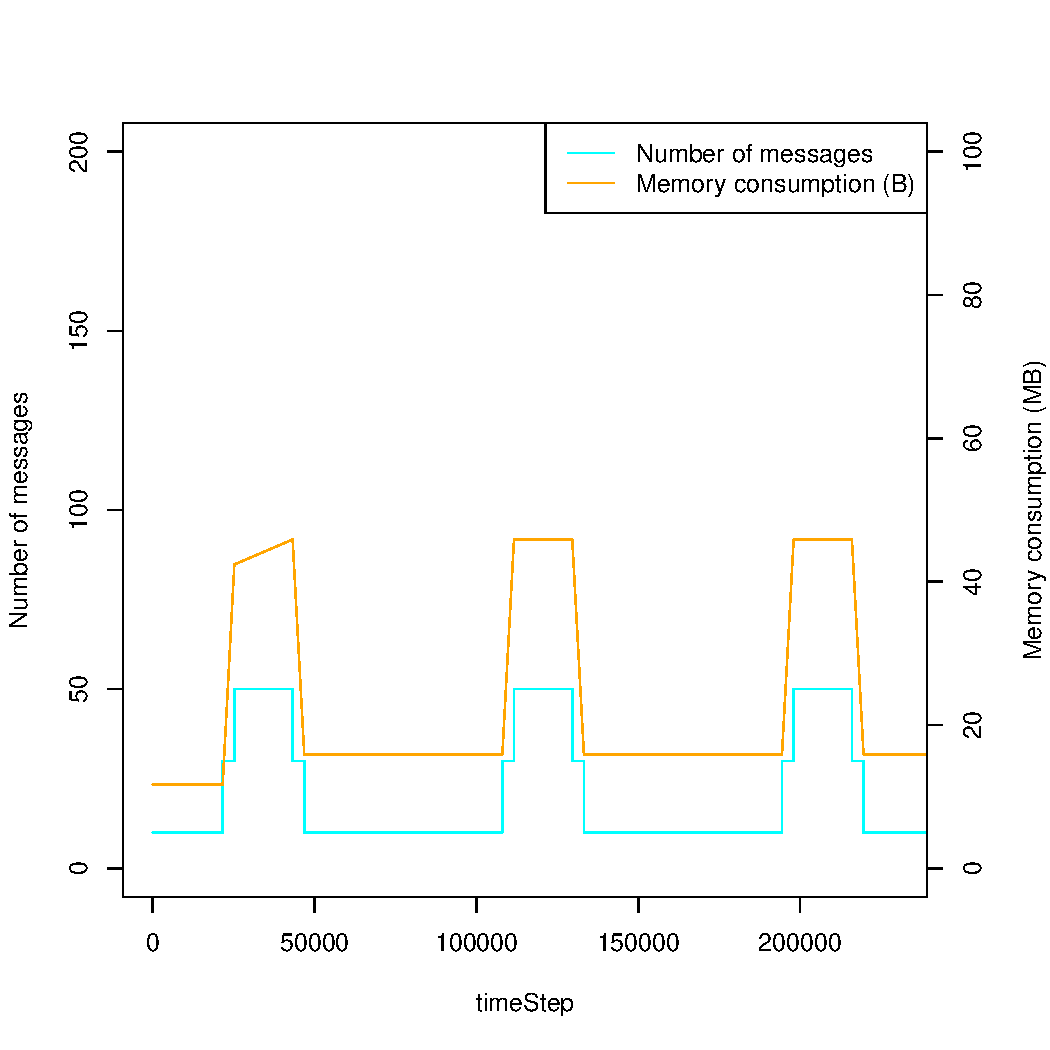
\includegraphics[width=0.6\hsize]{scenario_4_signaling_and_memoryload_vs_timeStep_all.pdf}
    \caption{メッセージ処理数とメモリ使用量の変化(シナリオ~3)}
    \label{scenario_3_signaling_and_memoryload_vs_timeStep}
  \end{center}
\end{figure}
\begin{figure}[htbp]
  \begin{center}
    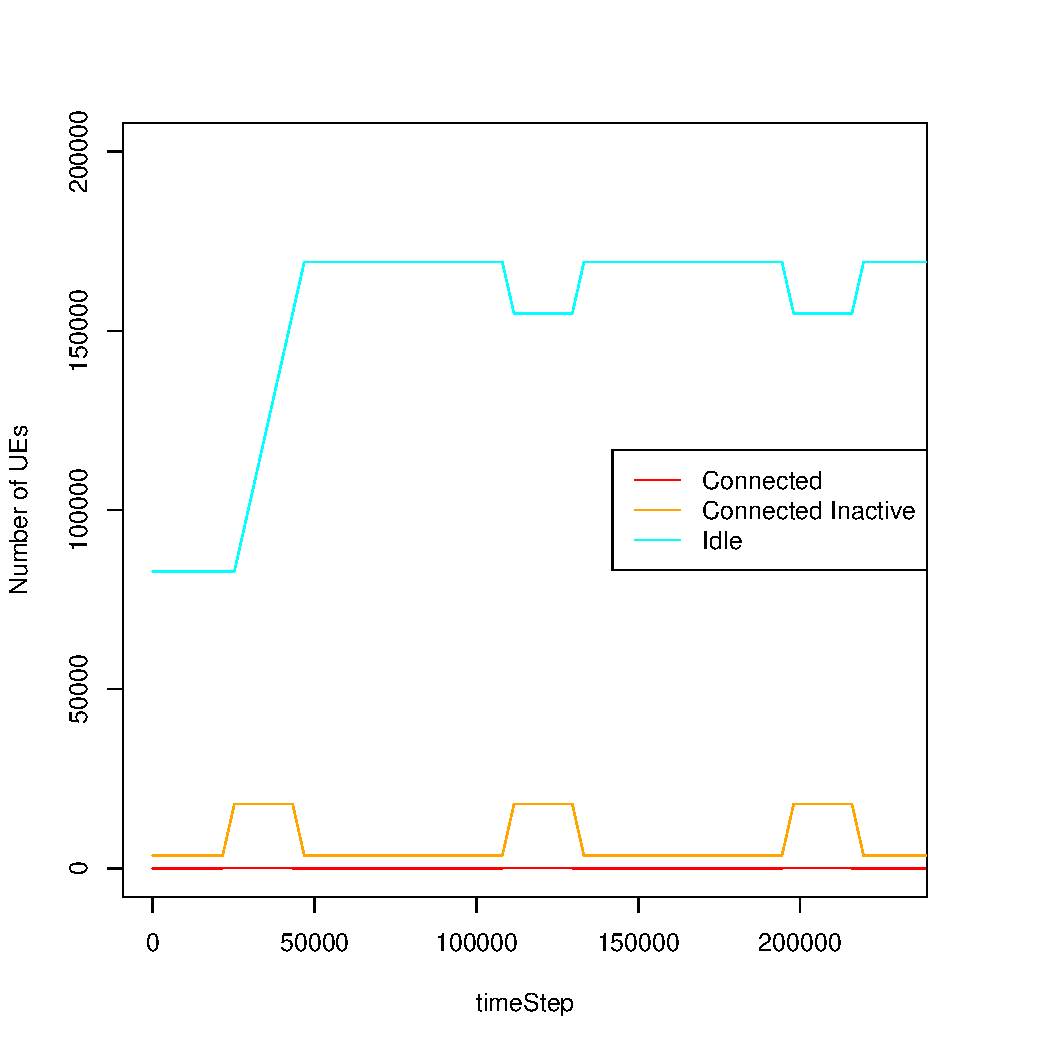
\includegraphics[width=0.6\hsize]{scenario_4_stateBreakdown_all.pdf}
    \caption{各状態に存在するUE台数の変化(シナリオ~3)}
    \label{scenario_3_stateBreakdown}
  \end{center}
\end{figure}
\clearpage

\section{今後の予定}
  \begin{itemize}
    \item PID制御に関する学習
    \item 発表スライドの作成: 〜10/18
  \end{itemize}
%
% \section*{\addcontentsline{toc}{section}{参考文献}}
% \bibliographystyle{IEEEtran}
% \bibliography{/Users/t-adachi/Documents/study/Bibliography/bib/hpt_core_network/myBib/LABbiblio,/Users/t-adachi/Documents/study/Bibliography/bib/hpt_core_network/Study_Group_Bibtex/bib/hptCoreNetwork_Study}
\end{document}
